
\begin{titlepage}

\begin{center}


\textsc{\LARGE Interdisziplinäre Projektarbeit 2012}\\[1.5cm]

\textsc{\Large Amsterdam}\\[0.5cm]

  
\HRule \\[0.4cm] 
{ \huge \bfseries Überflutung Hollands}
\newline
Holland wird sich von der nächsten grossen Flut nicht erholen können.
Frage: Ändern zu 100 Jahre. ist besser berechenbar. z.B was ist gross. wenn könnte gross sein. ist sehr schwer.
\HRule \\[0.4cm]  
  
 
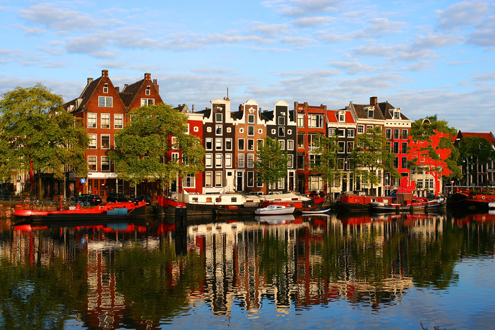
\includegraphics[width=1\textwidth]{images/titelbild.jpg}
\cite{titelbild} \text{Amsterdam: Houses along the Amstel River}  
\\[1cm]   
  
 
 
% Author and supervisor
\begin{minipage}{0.4\textwidth}
\begin{flushleft} \large
\emph{Autor:}
\\Claudia \textsc{Saxer}
\\Simon \textsc{Schneider}
\\Stefan \textsc{Kull}
\end{flushleft}
\end{minipage}
\begin{minipage}{0.5\textwidth}
\begin{flushright} \large
\emph{Lehrpersonen :} 
\\Dr.~Jose \textsc{Osuna}  \textnormal{Mathematik}
\\Frau \textsc{Wyss} \textnormal{Englisch}
\\Frau \textsc{Heckman} \textnormal{Geschichte}
\end{flushright}
\end{minipage}
\\[1.5cm]
\begin{minipage}{0.5\textwidth}
\begin{center} \large
\emph{Berufbildungsschule Winterthur}  
\\ \textsc{BMS I}
\\ \textsc{technische Richtung }
\end{center}
\end{minipage}

\vfill

{\large \today}

\end{center}


\end{titlepage}


